
\documentclass[a4paper,14pt]{extreport}
\usepackage[utf8]{inputenc}
\usepackage[T2A]{fontenc}
\usepackage[russian]{babel}
\usepackage{amssymb,amsfonts,amsmath}
\usepackage{multicol}
\usepackage{graphicx}
\usepackage{listings}
\usepackage{alltt}
\usepackage{verbatim}
\usepackage{listingsutf8}
\usepackage[
 left=25mm,
 top=20mm,
 right=10mm, 
 bottom=20mm, 
 nohead, 
 nofoot] {geometry}
\pagenumbering{arabic}

\parindent=0pt

\newcommand{\labtitle}{
 
}
\newcommand{\labnumber}{3}

\begin{document}
\title{Отчет по лабораторной работе \labnumber}
\author{Vladislav Tsisyk}
\thispagestyle{empty}
\begin{center}
\normalsize{Министерство образования и науки Российской Федерации}\\
\vspace{0.3cm}
\normalsize{Федеральное государственное бюджетное образовательное учреждение \\
высшего профессионального образования \\
«Алтайский государственный технический университет им. И.И. Ползунова»}\\*
\end{center}


\vspace{0.5cm}

\begin{flushleft} {
{\underline{Факультет Информационных Технологий}} \\
\vspace{0.2cm}
{Кафедра \underline{прикладной математики}} \\
\vspace{0.2cm}
}
\begin{tabular*}{\textwidth}{@{}l@{\extracolsep{\fill}}l}
~  &   Отчет защищен с оценкой \hrulefill \\
~ & Преподаватель \hrulefill\underline{\hspace{4cm}} Н.~Д.~Бубнова\\
~ & <<\underline{\hspace{0.8cm}}>> ~\underline{\hspace{3cm}} 2015 г.\\
\end{tabular*}

\end{flushleft}

\vspace{0.1cm}
\begin{center} {
\large{Отчет \\ по лабораторной работе №\labnumber} \\

\labtitle
}
\begin{center}
    I  семестр
 \end{center}
\vspace{0.4cm}

\linespread{0.7}{\Large{по дисциплине <<Введение в алгоритмы и основы технолог. разраб. пр.>>}}



\end{center}
\vspace{7cm}

\begin{center}

\begin{tabular*}{1.0\textwidth}{ll@{\extracolsep{\fill}}c}
Студент группы ПИ-41  & \underline{\hspace{6cm}}~В.~О.~Цисык & ~\\
Преподаватель \hfill & \underline{\hspace{6cm}}~Н.~Д.~Бубнова & ~ \\
\end{tabular*}
\end{center}

\vspace{\fill}

\begin{center}
\Large{БАРНАУЛ 2015}
\end{center}
\newpage

\textbf{Задание:}\\
Задан список чисел. Образовать из него новый, исключив из исходного
 минимальное число элементов так, чтобы список стал неубывающим
\subsection*{Описание алгоритма:}
Программа начинает свое выполнение с того, что запрашивает у пользователя файл с исходными данными.
Если файл с заданным именем существует, то создается пустой список, в который по очереди записываются исходные данные.
Список с исходными данными передается в функцию list\_LIS().\\ \\
Если список пуст(файл был пустым), то функция возвращает пустой список. Иначе, просматривается весь список. 
Во вспомогательный массив len записывается длина длиннейшей неубывающей подпоследовательности в списке до определенного элемента, 
len[i] - длина подпоследовательности на i-ом элементе списка. В массив prev записываются "позиции" элементов, при которых
подпоследовательность имеет наибольшую длину. \\ \\
После обработки списка, мы находим "элемент", при котором длина подпоследовательности - наибольшая. 
По массиву prev восстанавливаем элементы и записываем их в список. Возвращаем список в вызывающую функцию. Ответ получен. 
Результат записывается в файл. 
\subsection*{Код программы:}
\small
\begin{verbatim}
/* lab3.c */
/* Задан список чисел. Образовать из него новый, исключив из исходного
 минимальное число элементов так, чтобы список стал неубывающим */

#include <stdio.h>
#include "list.h"
#define LINELENGTH 1024
int main()
{
        FILE *fp;
    char line[LINELENGTH];
    char *p;
    int c, n;
    struct List *test = NULL;
    struct List *answer = NULL;
    test = list_init();
    printf("введите имя файла:");
    scanf("%s", line);
    if((fp = fopen(line,"r")) == NULL){
        fprintf(stderr, "Нет такого файла\n");
        return 1;
    }
    /* читаем строку за строкой */
        p = line;
    while(fgets (line, LINELENGTH, fp)){
         while(sscanf(p, "  %d%n", &c, &n) == 1 ){
                        list_insert(test, c);
             p +=n;
        }
    }
 
        answer = list_LIS(test);
        fclose(fp);

        while ((c = getchar())!= '\n' && c != EOF);/* отсеять всякий мусор */
        printf("Сохранить в файл? [y/n]:");
        scanf("%c", &c);/* пропустить пробелы и получить ответ */
        switch (c){
        case 'y': case 'Y': 
        printf("Записано в \"output.txt\"\n");
        fp = fopen("output.txt", "a");
        fprintf(fp, "------------------------\n");
                while(answer->head != NULL){
                        fprintf(fp, "%d ", answer->head->number);
                        answer->head = answer->head->next;
                }
        fprintf(fp,"\n");
        fclose(fp);
        break;
        }

        return 0;
}


/* list.c */
#include <stdlib.h>
#include <assert.h>
#include <stdio.h>
#include "list.h"

/* Сощдаем новый список */
struct List *list_init(void)
{
        struct List* theList = malloc(sizeof(struct List));
        assert(theList != NULL);

        theList->head = NULL;
        theList->tail = NULL;
        return theList;
}

/* Добавляем в конец списка */
void list_insert(struct List *test, int number)
{
        struct Node *newNode = malloc(sizeof(struct Node));
        assert(newNode != NULL);
        newNode->number = number;
        newNode->next = NULL;
        if(test->head == NULL)
                test->head = test->tail = newNode;
        else{
                test->tail->next = newNode;
                test->tail = newNode;
        }
}

/* Добавляем в начало списка */
void list_push(struct List *test, int number)
{
        struct Node *newNode = malloc(sizeof(struct Node));
        newNode->number = number;
        newNode->next = NULL;
        if(test->head == NULL)
                test->head = test->tail = newNode;
        else{
                newNode->next = test->head;
                test->head = newNode;
        }
}

/* Обрабатываем список  */
struct List *list_LIS(struct List *test)
{
        int *prev = NULL;
        int *len = NULL;
        struct Node *tmp = test->head;
        struct Node *first = NULL;
        struct List *answer = NULL;
        answer = list_init();
        int i,j, n;
        int pos, length;
        length = i =  0;

        /* пуст ли список? */

        if(tmp == NULL)
                return answer;
        while(tmp != NULL){

                /* выделить память под очередные элементы массива*/
                prev = realloc(prev, (++length) * sizeof(int));
                len = realloc(len, (++length) * sizeof(int));
                /* запомнить позицию головы */
                first = test->head;
                prev[i] = -1;
                len[i] = j = 0;

                /* находим количество элементов меньше определенного */
                while(first != tmp){
                        if(first->number <= tmp->number &&
                        len[j] + 1 > len[i]){
                                len[i] = len[j] + 1; 
                                prev[i] = j;
                        }
                        first = first->next;
                        j++;
                }
                /* printf("%d --- %d --- %d\n", len[i], tmp->number, prev[i]);*/
                tmp = tmp->next;
                i++;
        }
        /* находим самую длинную последовательность чисел... */
        n = length;
        pos = 0;
        length = len[0];
        for(i = 0; i < n; i++)
                if(len[i] > length){
                        pos = i;
                        length = len[i];
                }

        tmp = test->head;
        i = 0;
        /* ...и пихаем ее в список */
        while(pos != -1){
                for(i = 0; i < pos; i++)
                        tmp = tmp->next;
                list_push(answer, tmp->number);
                pos = prev[pos];
                tmp = test->head;
        }

        return answer;
}


/* list.h */

 struct Node{
        int number;
        struct Node *next;
};

struct List{
        struct Node *head;
        struct Node *tail;
};

struct List *list_init(void);
void list_insert(struct List *test, int number);

struct List *list_LIS(struct List *test);
void list_push(struct List *test, int number);


\end{verbatim}
\normalsize
\subsection*{Результаты тестирования:}
\begin{center}
	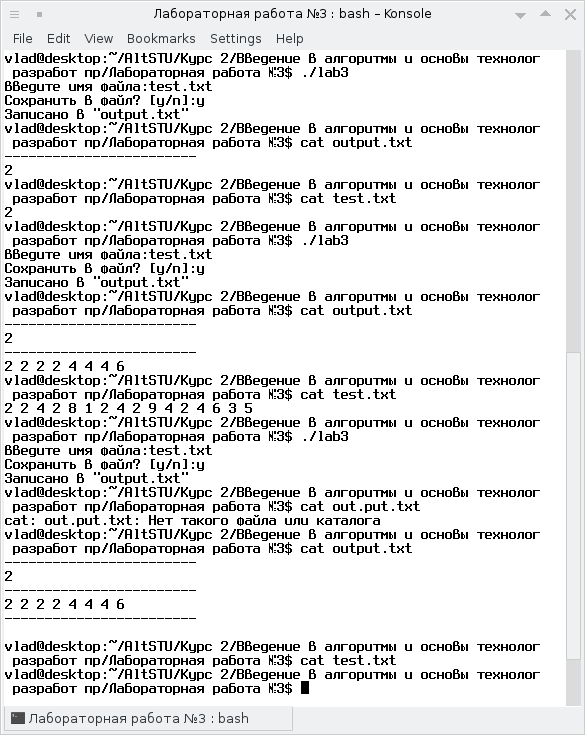
\includegraphics[scale = 1]{2.png}
\end{center}

\end{document}
